\chapter{More mechanics, more syntax}
\section{Introduction}
After the brief introduction of the last chapter, you probably have a bunch of questions, things like 
\begin{itemize}
\item    
The math-y stuff in double quotes --- what am I allowed to write in there? Can I use things like \isi{using} and \isi{show}? 
\item    
When do I need double-quotes? 
\item    
This whole \isi{using} thing seems annoying. Why doesn't Isabelle just keep track of the things I've proved and assume that I want to use those whenever possible? 
\item    
We used the name \isi{example} (and later the shorter \isi{ex} for the various facts we accumulated, but what are the rules for those? From trying out \isi{instance} I could see that using an Isabelle keyword was bad, but is everything else OK? 
\item    
How do I type the characters that I need? I can't just wait for you to tell me all of them!
\item    
You had me use \sys{Output} and \sys{State} in two of the panels, but what are those other things? 
\item    
Do I have to put everything in one theory file?
\item    
In all those proofs, you built up stuff to prove the main ``thesis'', but what about proofs where we work backwards from the thesis, like saying ``to prove that for positive integers $n$,  $2n + 1 > n + 1$, it suffices to prove  that $2n > n$''? Can we do those in Isabelle? 
\item    
Building up proofs in individual steps seems OK, but if a theory file gets big, how will I remember the names of all the things that I can use in trying to write a proof -- is it \isi{plus_commute} or \isi{add_commute}? Can Isabelle help with some of this?
\end{itemize}

We'll answer some of those in this chapter, and partially answer others. In making this list, I wanted to reassure you that if you feel confused about something, it's perfectly reasonable: Isabelle has a lot of parts, and it's impossible to introduce them all at once, so there'll be pending questions for a while.

\subsection*{Disclaimer}
By the way, Isabelle is a system in which something called Higher Order Logic (HOL) is implemented, resulting in Isabelle/HOL, which is what I've been calling ``Isabelle''. There are other logics implemented in Isabelle as well, such as First Order Logic, and Zermelo-Frankel Set Theory; these result in Isabelle/FOL and Isabelle/ZF, about which I will say no more because I know nothing about them. Furthermore, the interface we'll use is called Isabelle/jEdit, and it's a complex program in itself. But I'm going to be sloppy and use the word Isabelle for this editor, for the Isabelle/HOL language, and for the whole ecosystem. 

You can write a program that links to Isabelle, or even write code within an Isabelle theory document, or ask Isabelle to produce code that implements something that you've proved (in Isabelle) to be correct. I know nothing more about these topics than that they exist, so you won't learn about them in this book. 

\section{Warmup: more mechanics}
\subsection{Symbols}
Looking at the bottom of the center column of the interface, we see this:
\begin{figure} [h]
    \centering
    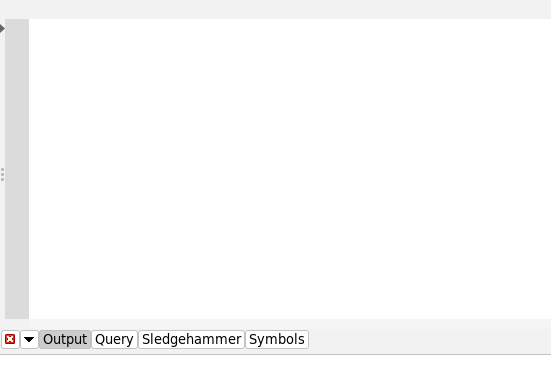
\includegraphics[width=0.5\linewidth]{C02//Images/image.png}
    \caption{A section of the interface}
    \label{fig:interface-section}
\end{figure}
\noindent
with \sys{Output} highlighted because we've been using this panel to see what's going on. 

But the \sys{Symbols} tab is also useful. Click on it, and you'll see a selection of choices:
\begin{figure} [h]
    \centering
    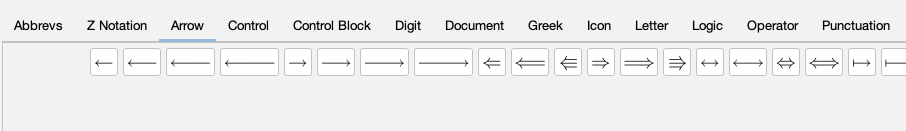
\includegraphics[width=0.75\linewidth]{C02//Images/symbols.png}
    \caption{The \sys{Symbols} panel has a bunch of options!}
    \label{fig:symbols-panel}
\end{figure}
\noindent 
where I've clicked on the choice \sys{Arrow}, which shows all the kinds of arrows available in Isabelle. If you move your cursor over one and let it rest there for a moment, a tooltip appears:
\begin{figure}
    \centering
    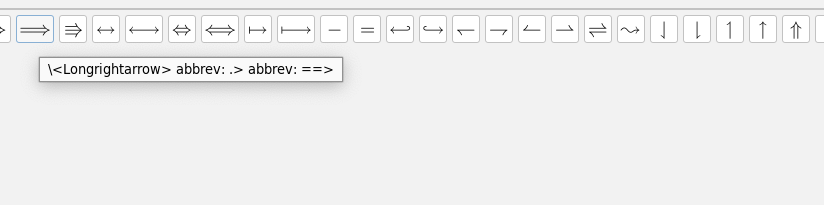
\includegraphics[width=0.5\linewidth]{C02//Images/tooltip.png}
    \caption{The tooltip for the double-right-arrow}
    \label{fig:double-right}
\end{figure}
and this tip this shows you that to produce that character in your theory file, you may type \verb|\\<Longrightarrow>| (although \isi{\\Longrightarrow} also works), or type ".>" (which doesn't work on my system), or type "==>", which does work. This lets you rapidly assemble a collection of shortcuts for symbols that you use often, and lets you look up others. If you use LaTeX, many of the symbol-names closely match the ones in LaTeX. The most useful of the options in this particular section is probably the one called "Search"; typing a few letters like \sys{sub} will show all symbols whose names contain that sequence, which makes it easy to find the symbol for \sys{subset}, for instance. Confession: I used this panel to find some favorite symbols, and now seldom look at it at all. 

In practice, I use only a few of the symbols, and below I show my go-to list. You've already seen greater-than-or-equal, and can guess at similar things, I'm hoping. And Greek letters are just given by their names with backslash in front, like \verb!\beta!.

\begin{longtable}{cc}
\caption{Favorite Isabelle symbols (needs work!)}\\
what you type & what you get \\ \hline
  \verb+[|+   & \isi{\\<lbrakk>} \\
  \verb+|]+  & \isi{\\<rbrakk>} \\

  \verb+\real+ &$\mathbb R$\\
  \verb+\int+  &$\mathbb Z$\\
  \verb+\nat+  &$\mathbb N$\\

  \verb+=>+  &\isi{\\<rightarrow>} \\
  \verb+==>+  &\isi{\\<Longrightarrow>} \\
  \verb+<>+   &\isi{\\<Longleftrightarrow>}\\

  \verb+EX+    &\isi{\\<exists>}\\
  \verb+ALL+   &\isi{\\<forall>}\\
  \verb+/\+    &\isi{\\<and>}\\
  \verb+\/+    &\isi{\\<or>}\\
  \verb+\not+  &\isi{¬}\\

  \verb+\equiv+ &\isi{\\<equiv>}\\
  \verb+\union+ &\isi{\\<union>}\\
  \verb+\inter+ &\isi{\\<inter>}\\
  \verb+\subset+ &\isi{\\<subset>}
\end{longtable}

\subsection{Query}
The \sys{query} tab gives you the ability to find already-proved theorems to use, saving you a ton of work. The only tricky thing about it is the need to press the \sys{Apply} button. So many other things in Isabelle's interface happen as you type that it's easy to forget. Within the Query panel are several choices:
\todo{fill in image here}

and the one that is probably most interesting to the beginner is "Print Context". If we take a simple theory like this one:
\todo{fill in image here}

with the cursor position shown in red, and check all four boxes (context, cases, terms, theorems) and press "Apply", we see this
\todo{fill in image here}

which helps disclose a little bit of what's going on during processing of a theory document. You can see that the name \isi{this} has been bound to \isi{n + 1 <= 2 * n + 1}, and \isi{?thesis} is bound to the same thing, and that there are some other 'facts' available for reasoning about goals. 
\task
Try moving the cursor up and down through a proof and clicking \sys{Apply} repeatedly to see a bit more. 
\etask
More useful in general is the \sys{Find Theorems} tab in this panel; we'll return to that somewhat later in these notes.

\subsection{Sledgehammer}
\term{Sledgehammer} is a proof-finding tool that applies a bunch of approaches all at once, spawning multiple processes; the chosen approaches are named in a list in the Sledgehammer tab. You can place your cursor somewhere in a theory where you need a proof (e.g., right after a theorem statement), and click the \sys{Apply} button in the Sledgehammer panel, and see the results. If in the example above I place my cursor right at the end of the lemma statement and use Sledgehammer, I'll see this produced over the course of a few seconds on my very slow old Macbook:
\todo{fill in image here}

As you can see, Sledgehammer is a lot like the "\isi{try0} that we've been using. But \isi{try0} does a lot less, so it operates faster, but with less power.  Sledgehammer is also, in my experience, one of the parts of Isabelle that's most likely to have failures of one sort or another, but you're unlikely to encounter these during early proving sessions. When you click \sys{Apply} in the sledgehammer panel, you're spawning a lot of computation…which continues until all the various solvers report back that they're done. This can slow things down a lot, so it's a good idea to click \sys{Cancel} as soon as you get tired of waiting or get a proof that you feel you can use. Sledgehammer will also sometimes report that one of its provers has found a proof…but then take forever to report what that proof actually is, or perhaps never do so. It'll also sometimes find a proof, but when you paste in that proof and Isabelle tries to use it, it takes too long and Isabelle reports a timeout. I'm just warning you that it can be frustrating! 

Pro tip: if you run sledgehammer, and then change something in the proof document \textit{before} the place where you're sledgehammering, then sledgehammer starts its work all over. You'll learn not to do this. You can also invoke sledgehammer, at a point where a proof is needed, by typing \isi{sledgehammer} right into your proof document, more or less the way you did with \isi{try0}. If you run sledgehammer in multiple places in your document, you may well run out of memory -- it's rarely a good idea. 

\section{Sessions}
\label{sec:sessions}
A single theory document is a place to put closely-related items, although the notion of 'closely-related' is of course ambiguous. Does everything about Group Theory go in one theory document? Or do we make a document for finite groups? Or perhaps a single document just for groups represented by generators and relations? That's all a matter of taste. But just as a book gets divided into chapters, there comes a time in the development of some mathematics when it begins to feel unwieldy. In Isabelle, this often happens at the time when loading your theory document starts to take a long time, during which all the initial work is checked even though you're planning to work only at the end. Wouldn't it be nice if you could take the completed part of your theory and store it away, and work on a new part that references that other portion? That's what 'sessions' are for. They serve much the same organizational function that directories/folders serve in a file-system: gather related items together in a hierarchical arrangement. There's a side-effect, though, one that's kind of nice: building a session also sets you up to be able to make a nice typeset version of your theory document. 

Fair warning: this discussion is something you'll read once, then apply by copying a few commands to set up a session, and then forget until the next time you need to do it. With that in mind, let's get to it!

All the files in a session are typically stored in a single directory, which contains all the related theory files and a special file called ROOT that describes the session. Every session has a \term{parent} (again like directories in a filesystem), except for the 'starting' session for Isabelle, called \isi{Pure} (the equivalent of the directory "/" on a Linux/Unix filesystem). The \isi{ROOT} file records the parent session. I'm only going to discuss the default structure for a session; fancier stuff is available in the documentation, but I've never needed it. 

Let's go ahead and create a session. I'll do this on my Macbook; you'll need to adapt things to your operating system. Things after \sys{//} are comments on what's going on; don't type them. All operations take place in a Terminal window. 

\digression[Paths]{sample text, because the actual text that follows is too long or something.}
{
On most systems, there's a notion of a search-path where the OS looks for programs to run. On linux-like systems, that typically involves things like "/bin". On my Macbook, it looks like this:
\begin{verbatim}
jfh@jfhs-MacBook-Pro book % echo $PATH
/Users/jfh/.npm-global/bin:/Library/Frameworks/Python.framework/Versions/3.11/bin:/usr/local/bin:/usr/bin:/bin:/usr/sbin:/sbin:/Library/TeX/texbin:/opt/X11/bin:/Library/Apple/usr/bin:/Users/jfh/.rvm/bin
\end{verbatim}

You can see that it's a list of colon-separated paths to various folders where executable programs are stored. If you type

\begin{verbatim}
% run-it foo
\end{verbatim}
\noindent
then the OS will search for a program called \sys{run-it} in all those places, and when it finds one, it will indeed run that program with \sys{foo} as a command-line argument. If it doesn't find that name anywhere, it'll say something like \sys{run-it: not found}. Isabelle itself has several runnable programs; on a Mac, they're found in \sys{/Applications/Isabelle2023/bin}; one of them is called \sys{isabelle}.You can add \sys{/Applications/Isabelle2023/bin} to your path so that this program can be found, or you can, in your Terminal program, change to the directory called \sys{/Applications/Isabelle2023/bin} and type 
\begin{verbatim}    
% ./isabelle
\end{verbatim}

to run it, or you can type the full name of the program, i.e., 
\begin{verbatim}
% /Applications/Isabelle2023/bin/isabelle
\end{verbatim}    

All three work. I'll use the last of these. 
}

\textbf{End of what should have been a digression}

Let's continue and use \sys{isabelle} to create a session:
\begin{verbatim}      
        // create a session on the desktop; be sure 
        //that ~/Desktop/book doesn't already exist!
% /Applications/Isabelle2023.app/bin/isabelle mkroot ~/Desktop/book  

Initializing session "book" in "/Users/jfh/Desktop/book"
  creating "/Users/jfh/Desktop/book/ROOT"
  creating "/Users/jfh/Desktop/book/document/root.tex"
Now use the following command line to build the session:
  isabelle build -D /Users/jfh/Desktop/book
\end{verbatim}

At this point the \sys{book} directory contains a text-file, \sys{ROOT}, and a subdirectory, \sys{document} with a LaTeX document \sys{root.tex} in it. 

\begin{verbatim}
    
        // Follow the instruction on the last line to "build the session"
% /Applications/Isabelle2023.app/bin/isabelle build -D /Users/jfh/Desktop/book
Running book ...
Preparing book/document ...
Finished book/document (0:00:28 elapsed time)
Document at "/Users/jfh/Desktop/book/output/document.pdf"
Finished book (0:00:02 elapsed time)
0:00:44 elapsed time
\end{verbatim}

As you can see, that last step is a little slow. So what happened? A bunch of stuff. If we go to the newly-created session, we see this:
\begin{verbatim}
jfh@jfhs-MacBook-Pro bin % cd ~/Desktop/book
jfh@jfhs-MacBook-Pro book % ls
ROOT		document	output
\end{verbatim}

Running the \sys{build} created a new \sys{output} directory, and the entire directory structure is now this:
\begin{verbatim}
    
jfh@jfhs-MacBook-Pro book % ls -R  
ROOT		document	output

./document:
root.tex

./output:
document	document.pdf

./output/document:
comment.sty			isabelletags.sty		root.tex
isabelle.sty		pdfsetup.sty		session.tex
isabellesym.sty		railsetup.sty		session_graph.pdf
\end{verbatim}

The contents of the ROOT file are this:

\begin{verbatim}
jfh@jfhs-MacBook-Pro book % more ROOT 
session book = HOL +
  options [document = pdf, document_output = "output"]
(*theories [document = false]
    A
    B
  theories
    C
    D*)
  document_files
    "root.tex"    
\end{verbatim}

What that's saying is that this session's parent is \sys{HOL}, for which Isabelle already has a precompiled \term{heap file}, which is its way of storing the results of processing all the theory files so that it can load them almost instantly rather than working through each one of hundreds of individual files. Processing a session also creates a heap file -- i.e., it creates a record of everything that results from processing the theory files in that session so that they don't all need to be re-loaded and processed, as mentioned in the previous chapter. The ROOT file also says that in creating a pretty document for this session, I want the result to be a pdf, and that this pdf should be put in the folder \sys{book/output}. It then, in a comment-block, shows how we might say which theory files are included in this session. In this case, it's indicating that theories A and B should not appear in the output document, but C and D should. And finally, it says that the files used to produce the output document (aside from the theory files themselves) are … well, there's only one, called \sys{root.tex}. If you wanted to include a bibliography, you might include 
sys{root.bib}, for instance. 

If we navigate to the "output" folder and look at the resulting "document.pdf", it's pretty boring:

\todo{show the pdf here}

but that's because there are no theory files in the session. Let's do one more thing, and include our chapter-zero theory file. Let's move that file from wherever you put it to the \sys{book} folder and then again run the \sys{build} process. In my case, the chapter-zero file was in my home directory:
\begin{verbatim}
jfh@jfhs-MacBook-Pro book % mv ~/IbookCh0.thy .
jfh@jfhs-MacBook-Pro book % /Applications/Isabelle2023.app/bin/isabelle build -D ~/Desktop/book   
0:00:11 elapsed time
\end{verbatim}

The result is … no change at all in the document.pdf file! That's because we didn't edit the ROOT file to tell it that our session had a new theory. We have to edit that file (use your favorite text-editing tool) to make it look like this:

\begin{verbatim}
session book = HOL +
  options [document = pdf, document_output = "output"]
  theories IbookCh0
  document_files
    "root.tex"    
\end{verbatim}

Notice that in listing the theories, I have to not include \sys{.thy} in the name! 
Then we can re-run the \sys{build} command and get a document.pdf that starts like this:

\todo{show resulting document here}


Warning: If your theory file contains an error, it's possible that your \sys{build} will fail, and then you need to fix things. If your document contains clever LaTeX tricks, debugging the build process can become a serious challenge, alas. I have no suggestions except that in trade for the beauty of the output, you have to eventually get comfortable with the challenges of the complicated LaTeX typesetting system.

That was a lot of mechanics, but we've mostly addressed items 5, 6, and 7 from the pending-questions list. 

\subsection{Encouragement}
In these first two chapters, I've introduced you, very slowly and carefully, to the mechanical parts of Isabelle that took me a while to learn, or surprised me, or were tricky (like getting the whole LaTeX thing set up). There will be more as we go along, but I encourage you to poke around in the interface for yourself and discover new things. For some, you'll probably ask ``Why would I even need \textit{that}?''; for others, you'll say ``Finally! That's just what I was hoping to find!'' 


There's one tip I can give here: the menus associated with the Isabelle interface (which is written atop something called \co{jEdit}) are almost all about \co{jEdit}, and therefore mostly uninteresting to beginning users. The thing that \textit{is} interesting and Isabelle-specific is in the \co{Plugins...Isabelle} menu, although I doubt you'll find much use for it until you're working on much more complex projects.


\section{More proving: a different style}

Let's move on to some more questions about actually proving things. 
Isabelle (and in particular Isar) provides another way of stating theorems, one that has a lot of appeal because of its consistency. For our little \isi{evens} theorem, it looks like this:
\begin{IS}    
lemma evens5:
  fixes k::nat
  shows "∃ n . 2*n > k"
proof -
  show ?thesis by presburger
qed
\end{IS}

I've used the simple presburger proof here so that I can concentrate on the statement. For more complicated theorems, there can also be an \isi{assumes} between \isi{fixes} and \isi{shows}. But in this simple case, the name \isi{k}, which was previously universally quantified without our saying anything about it, is made explicit up front. This is meant to remind you of the way you might start when you want to show that ``for any $k$, there's an even number bigger than $k$.'' You start by saying ``Let's fix some arbitrary natural number $k$, and then …'' 

\subsection*{Getting theorem statements right, and how Isabelle can help you}
Let's suppose you want to show that for positive $n$, we have $2n + 1 > n + 1$, and you write

\begin{IS}
lemma "dominate": "2* (n::nat) + 1 > n + 1"
  by presburger    
\end{IS}
\noindent
filling in the \isi{by presburger} based on your experience with showing this sort of thing.  Go ahead and type this in, and see what happens. 
\todo{picture here}
You'll notice two things: the proof has a red circle to its left, with  \isi{presburger} underlined with a red squiggle, and the theorem itself has a blue `i' next to it. If you place your cursor on the lemma statement, you'll see in the output window 
\todo{Show the nitpick output}

That's telling you that a background process has been checking the theorems you're claiming, just to see whether it can find an easy counterexample. In this case, it came up with $n = 0$, which is indeed a natural number for which the alleged theorem's not true. This can be a big help in getting theorem statements right. 

We can restate that ``dominate'' lemma in fix-assume-show form:
\todo{include example here}
My experience is that this structure helps me remember to assign types to things (in the \isi{fixes} line), and to write down all hypotheses (in the \isi{assumes} line). I've omitted writing a proof because I want to use this example later to show a different style of proving from the ones we've seen so far. 

There's a corresponding proof structure to the theorem-stating \isi{fixes-assumes-shows} pattern. It uses the imperative form of the three verbs: \isi{fix, assume, show}. We'll return to this in Chapter XXX.

Each of the three parts of a \isi{fixes-assumes-shows} theorem-statement can also contain \isi{and}, or can be repeated, so \isi{fixes n and k} is acceptable, but so is 
\begin{IS}
  fixes n 
  fixes k    
\end{IS}

Here's a very silly example making two claims about some natural numbers, showing how 
\isi{and} is used. 

\todo{insert examples here}

Two notes are due here.

Generally showing two or more things isn't a great idea. When you later refer to the theorem, Isabelle has to guess which conclusion you think is relevant in the current situation. Of course, if there's some complicated set of hypotheses that you don't want to repeat multiple times, and that leads to several facts (e.g., a theorem of the form "If we know A, B, and C, then the following 5 statements are all equivalent"), it's OK to write such a theorem. But don't do it unless you need to. (To be fair, I'll be violating this first suggestion in a page or two!)

If in my silly lemma I had replaced the second conclusion with "n * k > 15", I'd have been stuck -- nothing we've learned about yet shows how to prove such an inequality. I'm deliberately concentrating for now on the \textit{structures} of proofs rather than the use of existing theorems to prove new ones. 

\section{Practice}
You're now going to practice writing theorems using the fix/assume/show format, and then proving them using the few tools you've learned so far. Thus the bulk of this Chapter's content is actually in an Isabelle theory file, one that needs to be filled in (by you!). 

To supply a meaningful example, I've taken part of the first chapter of Michael Spivak's Calculus, which introduces an axiomatic formulation of the real numbers, and encoded it in Isabelle. (The book, at least in early editions, is widely available as a PDF download.) Spivak shows how to use the axioms to prove some small results, and I've imitated some of those proofs (almost verbatim) in Isabelle.

\task Find Spivak's book and open up that first chapter so that you know what we're talking about for the remainder of this chapter. 
\etask

Open up the \co{IbookCh1_starter.thy} file and take a look at the first few lines, and then continue reading here.

One challenge here is that the natural numbers and integers, and their associated notions of addition and multiplication are already present in Main, and I want to be sure that Spivak's discussion isn't polluted by those. To do so, I've declared a new type, named \isi{r} (for "real"), to serve as a proxy for the real numbers. When we declare a new type, we're guaranteed two things: there is at least one value of that type, and any value of our new type is different from any value of any previously-existing type. So it gives us a clean slate to work from. 

Initially we know virtually nothing about the type \isi{r}, but I've used the \isi{sorry} feature of Isabelle to allow me to make statements about elements of \isi{r} that will be taken as true henceforth. Yes, I warned earlier about the perils of \isi{sorry} and how one might accidentally introduce inconsistent 'truths' by using them. But I'm pretty confident that the axioms of the reals are not, in fact, contradictory, so I'm happy to do this for this example. 

By the way, statements to be taken as true henceforth are called \term{facts}. 

There's an alternative Isabelle construct -- axiomatization -- that I could have used for the same purpose, but it's generally reserved for quite specific tasks like defining a new logic, and I don't expect to ever use it in my Isabelle documents, so I wanted to avoid using it here. Let's see how things start out:

I've said here that there's a new type called \isi{r}, and that there are six "constants". The first four are functions called \isi{plus, minus, neg,} and \isi{reciprocal}; the last two are single elements of \isi{r} to which I've given the name \isi{Z} (suggesting 'zero') and \isi{U} (suggesting 'unit', and which is supposed to act as 'one' in our number system, but abbreviating with the first letter and getting "O" seemed like a really bad choice for something that was representing "1"). A constant is simply a name that will be used throughout a document to mean a single thing. \isi{True} and \isi{False} are constants of type \isi{bool}, for example. By the way, although we've given the names \isi{Z} and \isi{U} to two items of type \isi{r}, they might actually denote the same item; nothing we've said so far prevents this.

In a \isi{consts} declaration in Isabelle, the name of each constant is given, followed by a double-colon, and then the type of the constant. This type-description must be in double-quotes unless it's particularly simple (as it is for \isi{Z} and \isi{U}). What about those arrows, though? 

Let's start with \isi{neg}, which is going to play the role of negation, i.e., producing the additive inverse of a number. Its type is \isi{r \\<Rightarrow> r}  (you produce the pretty arrow shown above by typing '\isi{=>}', and in this text document I'll continue to use that). What \isi{A => B} means is that this thing is a function taking an argument of type \isi{A} to a result of type \isi{B}. If you like, \isi{A} is the domain and \isi{B} is the codomain. (There's a subtle point here: \isi{A} is a \textit{type}, not a \textit{set}. So there's no way in this format to describe a function from the even integers to the positive reals, for example.) The \isi{neg} function has type \isi{r => r}, meaning that it takes in an item of type \isi{r} (which we're thinking of as a real number) and produces an item of type \isi{r}.

\digression[types]{ I'm slowly introducing the language of types in Isabelle. There are several that are in Main (like \isi{int} and \isi{nat}), but you can create new types (i.e., labels to use for things to be certain that they're treated as different from anything else that is not of that type) using \isi{typedecl}. You can also describe a new type by writing \isi{type1 => type2}, which is the name for the type of things that are functions from \isi{type1} to \isi{type2}. (Some people call these \term{arrow types}.) So \isi{nat => nat} is a type that you could assign to some name. Given that you can put an arrow between any two types, you could write \isi{int => nat => nat}, which Isabelle treats as \isi{int => (nat => nat)}, i.e., if \isi{f} has this type, then \isi{f 3} denotes a nat-to-nat function. Just to clarify: in Isabelle, \isi{f 3} denotes what, in mathematics, we'd write as $f(3)$. And that's enough about types for the moment.} 

As observed in the digression above, in Isabelle, function names are followed by arguments, so while in a mathematics text we might write $f(x)$, in Isabelle we'd write \isi{f x}. That takes some getting used to. This means that if we want to think about the additive inverse of the multiplicative identity element, we'll need to write \isi{neg U}.

Now let's look at \isi{plus}. Most mathematicians would say that \isi{plus} is a function from $\mathbb R \times \mathbb R$ to $\mathbb R$. \rsdone{should there be only two $\mathbb R$'s on the left?} Let's call that function $p$ for the moment, so that $p(3, 5)$ denotes the sum of $3$ and $5$. We could define a new function, $q$, by saying that $q(x) = p(3, x)$, right? Then $q$ would be the ``add 3'' function. And we could define $h$ by $h(x) = p(14, x)$, so that $h$ is the ``add 14'' function. Clearly we can generalize like mad and define $S(a)$ to be the function sending $x$ to $a + x$. This process is called "currying", and computer scientists love it. (The term is named for Haskell Curry.) In this example, the domain of $S$ is "reals" and the codomain is "real-to-real functions". If we adopt the notation $A => B$ to denote all functions from $A$ to $B$, then the function $S$ has the type
$\mathbb R \Rightarrow (\mathbb R \Rightarrow \mathbb R) $. Computer scientists would write that as \isi{r => r => r}, saying that ``=>'' 'associates to the right', so that the parentheses are unnecessary. \marginnote{In Isabelle, all arrows associate to the right, which is useful to remember. If you're feeling unsure, you can add parentheses to clarify things, but eventually you'll get tired of adding them and just remember the rule.}

And that's what our declaration of 'plus' is saying: 
\begin{IS}
plus:: r => r => r
\end{IS}

Thus \isi{plus 3} is the function sending \isi{x} to \isi{3 + x}, and \isi{plus 3 5} applies this function to the number \isi{5}, and hence it evaluates to \isi{8}. Or at least all that would be true if we defined plus properly, and if \isi{3} and \isi{5} were actually names for things of type \isi{r}. But anyhow, that's the intuition. So our first few lines say that we have functions that will represent addition, multiplication, additive inverse, and reciprocal. 

You're going to quite reasonably object that zero does not have a reciprocal. Unfortunately, all functions in Isabelle are "total" -- they're defined for every value of the domain type. But in our case, we're not going to actually define reciprocal -- we're going to say some properties that it has. And none of those properties will be ascribed to zero, so while \isi{reciprocal Z} is legal to write, we cannot say anything about it. This takes some getting used to, and for now I encourage you to just let it roll past you and accept that it probably works or this whole Isabelle project would have crashed to the ground two decades ago. 

On to the next two lines:

We're used to writing $3 + 5$ instead of $\operatorname{plus}(3, 5)$; this is called \term{infix} notation, because the position of the operator (namely $+$) is fixed to be in the middle of the operands. Negation uses "$-$" as a "prefix" operation. And if you ever used an HP calculator or an adding machine, you're used to entering something like \verb!3 <enter> 5 +! and seeing the result \verb!8!. This is called \term{postfix} notation, because the operator comes post-operand(s). Isabelle's \isi{notation} command is used to say (in the first line) that if we write \isi{Z \\<oplus> Z}, that is to be interpreted as \isi{plus Z Z}. There's a whole question about what 
\isi{A \\<oplus>B \\<oplus> C} might mean, and whether addition binds more tightly than multiplication or vice-versa; the number \isi{80} \rs{Why 80?} above says that our two new operations "bind fairly tightly", so that \isi{U = Z \\<oplus> Z} is interpreted as the false statement that one is zero plus zero, rather than as an attempt to add the boolean value \isi{U = Z} to the \isi{r}-value \isi{Z}. In general, if we run into a situation where an infix operation seems to be causing trouble for Isabelle, parentheses help, so \isi{U = (Z \\<oplus> Z)} is unambiguous regardless of operator precedence. 

That was a whole lot of description for just 10 lines of a theory document. It'll get better. 

Spivak begins by talking about adding pairs of numbers, and then about adding up three numbers, noting that one could define addition of any number of numbers, but that it was simpler to just say how to add two of them, and then use this to add up three, by saying that $a + b + c$ should be interpreted as $(a + b) + c$, i.e., first add $a$ and $b$; then add the result to $c$. But there's another possible choice that could be made, namely that $a+b+c = a + (b+c)$. And he then says that ensuring these two are the same is the first thing we want in our number system, and calls this property P1. I've written this as an un-proved lemma: 
\begin{IS}
  lemma plus_assoc: (* Spivak calls this P1 *)
  fixes a::r and b::r and c::r
  shows "(a ⊕ b) ⊕ c =  a ⊕ (b ⊕ c)"
  sorry
\end{IS}

In my "fixes" line I've given types to a, b, and c. I could have omitted the types of all three because in the "shows" line they get the ⊕ operation applied to them, so they must be of type \isi{r}. In general, Isabelle documents omit type annotations like the ones I've provided, but these annotations do no harm, especially if they're used sparingly. For this starter material, I'm trying to be generous with clarifying everything for you. In a week or so, you'll find yourself thinking how stupid that was and how cluttered these early proof documents look. 

\subsection{A quick introduction to unification}
How does Isabelle know that these things have to be of type \isi{r}? Through an algorithm called \term{unification}. Suppose that the \isi{fixes} line was \isi{fixes a and b and c}. From the \isi{fixes} line Isabelle knows that \isi{a, b}, and \isi{c} have some unspecified type. Let's call that type `alpha', which programming-language folks write as \isi{'a}, so that they can use ASCII; they use \isi{'b} for beta, and \isi{'c} for gamma, and so on. In fact, all we know at this point is that \isi{a} has some type \isi{'a}, \isi{b} has some type \isi{'b}, and \isi{c} has some type \isi{'c}. It's possible that \isi{'a = 'c}, but at present we don't know. 

In the \isi{shows} line, we have \isi{plus (plus a b) c = ...} But when we defined \isi{plus}, we said it was an \isi{r => r => r} procedure, so its first argument has to have type \isi{r}, so does its second argument, and so does the result. So at this point we know:
\begin{longtable}{cc}   
Item             & type \\ \hline
\isi{plus}  &              \isi{r => r => r}\\
\isi{a}     &            \isi{'a}\\
\isi{b}       &           \isi{'b}\\
$\to$\isi{c}        &          \isi{'c}\\
\isi{(plus a b)}&         \isi{r}\\
$\to$\isi{c}          &         \isi{r}\\
\isi{plus (plus a b) c} &  \isi{r}    
\end{longtable}
(Make sure you understand why we know each of these things, given what's been said so far). A little terminology here: things that have types are called "\term{terms}, so our table's first label should really be ``Term'' rather than ``Item''. 

The two marked terms both assign a type to the term \isi{c,} so these types must be equal. Hence the previously-unknown type \isi{'c} turns out to be \isi{r}. If you like, we have an equality of types, \isi{'c = r}. And we could similarly write down a bunch more equations and "solve" the system of type-equations. But in practice, immediate substitution works fine in a case like this. So making this first replacement,  we arrive at:
\begin{longtable}{cc}   
Item             & type \\ \hline
\isi{plus}  &              \isi{r => r => r}\\
\isi{a}     &            \isi{'a}\\
\isi{b}       &           \isi{'b}\\
\isi{c}        &          \isi{r}\\
\isi{(plus a b)}&         \isi{r}\\
\isi{c}          &         \isi{r}\\
\isi{plus (plus a b) c} &  \isi{r}    
\end{longtable}
There's another term to consider: plus a b. Because of the type-signature for plus, we know that a, b, and plus a b must all have type "r", so our table expands with three more equations.
\begin{longtable}{cc}   
Item             & type \\ \hline
\isi{plus}  &              \isi{r => r => r}\\
\isi{a}     &            \isi{'a}\\
\isi{b}       &           \isi{'b}\\
\isi{c}        &          \isi{r}\\
\isi{(plus a b)}&         \isi{r}\\
\isi{a}     &            \isi{r}\\
\isi{b}     &            \isi{r}\\
\isi{c}          &         \isi{r}\\
\isi{plus (plus a b) c} &  \isi{r}    
\end{longtable}
The term \isi{b} now has both types \isi{r} and \isi{'b}, so these must be the same, and a similar thing applies to the term \isi{a}. Making these substitions gets us a table 
with no more terms of undetermined type. In this toy example, there's really only one main type (r), but in general, this matching up of types can be pretty important, and goes by the name \term{unification}. 

By the way, unification is `finished' when there are no more substitutions to be made. That doesn't mean that every type-variable like 'a or 'b has been unified with some known type; it just means that no more progress can be made. 

Analogously, in this system of equations over the reals:
\begin{align}
x + y + 2z &= 3 \\
x + y + 4z &= 5
\end{align}
We can subtract the first from the second to get 2z = 2, hence z = 1, and simplify to 
\begin{align}
x + y &= 1\\
x + y &= 1
\end{align}
\noindent
which reduces to a single equation which has many possible solutions, i.e., $x$ and $y$ remain 'unknowns'. 

\subsection{Lemma-processing, continued}
Following the processing of this lemma, we know that
\begin{IS}
(Z \<oplus> U) \<oplus> U = Z \<oplus>  (U \<oplus> U),
\end{IS}for instance. We could, in a later proof, assert this as a claim, followed by \isi{using plus_assoc by auto} as a proof. This, too, is somewhat like unification: we have a proposition that says that if you have a term that "matches" (i.e., has the general form) 
\begin{IS}
   (something1  \<oplus> something2)  \<oplus> something3
\end{IS}
then you can replace it with the same things, but parenthesized in the other way. In our case, we \textit{do} have a match: \isi{Z} serves as \isi{something1}, \isi{U} serves as \isi{something2}, and \isi{U} again serves as \isi{something3}. 

Informally, that's (very loosely speaking) what's going on as Isabelle tries to get from your collection of known facts (i.e., hypotheses and previously shown facts) to your conclusion(s): it tries to match up the structure and types of some fact with those in the assumptions of some lemma, and then add the conclusion of the lemma to your collection of facts. We suggest the lemma (or other known relationship) that should be used for the matching-up by \isi{using}, and in what we've seen so far, the matching up is done by \isi{auto}. And right now, we're doing all the work: we decide what fact to assert next, look for the supporting proposition that 'matches' it and put that name after \isi{using}, and then say \isi{by auto} (or sometimes \isi{by blast}). 

Sometimes we can get away with two steps at once. Suppose we wanted to show that 
\begin{IS}
(Z \<oplus> U) \<oplus> U = U \<oplus>  (Z \<oplus> U).    
\end{IS}
The argument might be that in \isi{(Z \\<oplus> U) \\<oplus> U}, we can swap the positions of the first two items to get \isi{(U \\<oplus> Z) \\<oplus> U}, and then use our associativity result to get the conclusion. Perhaps we have a \isi{plus_commute} lemma. We could then say \isi{using plus_assoc plus_commute by auto} in the proof. But \isi{plus_commute} can be applied all over the place! In that first expression,
\begin{IS}
(Z \<oplus> U) \<oplus> U    
\end{IS}
we can use it to transform things to \isi{(U \\<oplus> Z) \\<oplus> U}, or to transform to \isi{U \\<oplus> (Z \\<oplus> U)}. If we did the second, then we couldn't apply \isi{plus_assoc} any more, though. We could also apply \isi{plus_assoc} first, and then apply \isi{plus_commute} in various ways to the result. There is, in the words of Jorge Luis Borges, a ``garden of forking paths'' here, and finding the one that leads from what we know to what we want becomes a kind of search problem: finding a path through the graph whose nodes are knowledge-states and whose edges are "transitions gotten by applying theorems or other facts" to these, a path that goes from our initial state of knowledge to one in which our desired conclusion is a known fact. There are 
\begin{itemize}
    \item Lots of dead ends in such a search
    \item Often multiple paths from our initial state to some goal state
\end{itemize}
\digression[The syntax for `using'.]{ Note that you can (and often will!) need to marshall several facts to prove something. While you might write \isi{have ... using fact1 using fact2 using fact3 by auto}, you can combine multiple facts into a single \isi{using}, as in 
\isi{have ... using fact1 fact2 fact3 by auto}. Here (as in the future) the \isi{...} stands for some portion of the theory file that I've deliberately omitted to focus on the thing I'm talking about. Many books do something similar, replacing \isi{by auto} with \emph{proof}, which is more generic (maybe your proof is \isi{by blast}, or maybe it's 20 lines long!), but which I found baffling as I first tried to learn Isabelle. The point here is that the \isi{by auto} is a proxy for some potentially more complex proof, but I find it nice to have something that \textit{looks like} a proof in that position.}
The first of these means that Isabelle's basic reasoning methods, which use a bounded number of steps, can't make very big leaps for us. In much of what we'll do initially, we'll be asking it to follow just one edge or maybe two in this graph. The second one means that if you use a fancy tool like sledgehammer, different solvers may come up with different ways to get to a solution, some of them quite short (\isi{by auto}) and others long and complex. 

With all that in mind, I'm now going to ask you to use Isabelle in this `baby steps' mode, where you take some known fact(s) and slightly transform it by applying a theorem/lemma/definition to get a new fact, gradually reaching your desired conclusion. The ``known fact'' is often the assumptions of the theorem you're trying to prove (and Isabelle gives it the name \isi{assms}), so you'll often write something like 
\begin{IS}
   have   1:"a \<in> P" using assms by auto 
\end{IS}

That's because the lemma you're trying to prove looks like
\begin{IS}
   fixes ...
   assumes "a \<in> P" and "b \<in> P"
   shows ...
\end{IS}
Once you've written that \isi{have}, you've got a named fact, namely that ``a is positive''; the name of the fact is "1" because you wrote \isi{have 1: ...}, which assigned that name. You can then, in a subsequent step, say something like
\begin{IS}
   have 2: "..." using 1 by auto
\end{IS}
to refer to fact 1. This `name every step' approach is not beautiful Isabelle style, but it's a good starting point from which we'll return in a \term{polishing} discussion of how to make your theories prettier. 

So go ahead and open up the theory file called \sys{IBookCh1-exercises.thy}, and start working through it. 

What follows in the document is a transcription of Spivak's text, with some omissions, and interleaved with some comments from me (prefixed with \isi{jfh: }) and some exercises for you to carry out (introduced with \isi{EXERCISE}). In each case you are asked to prove some statement. Spivak's text, and my notes and exercise-announcements, are written within a block of text that looks like \isi{text < ... >}, which is material that would appear in a PDF of this proof document if you did the steps described in Section~\ref{sec:sessions} 

Doing each exercise entails writing a lemma with a name like "ex1" (for "exercise 1") in fix-assume-show format and then 
constructing a proof that's analogous to one you've seen previously in Spivak's text. 

Much of the time \isi{using <something> by auto} will suffice for proving individual things that arise in the proof. If you get frustrated, \isi{try0} may help you; chances are good that you forgot to include \isi{assms} in the \isi{using} clause. If all else fails, you can use \isi{sorry} and move on to the next exercise. 

I've already mentioned that Isabelle is constantly doing many things in many threads of execution. There's another thing going on, too: when you defined something, like
\begin{IS}
    definition my_add where "my_add p q = p + q + (1::nat)"
\end{IS}
which defines a \isi{nat => nat => nat} function, not only does that allow you to use that function henceforth, it also adds a \term{fact} to the world, something that can be used when you want to write \isi{using ...}; that fact is named \isi{my_add_def}, i.e., the name of the function followed by the characters \isi{_def}. You'll find yourself using these facts a lot as you do these exercises. 

You should continue on with at least the remaining material discussing P1 -- P9, but omitting the material after the proof that $(-a)(-b) = ab$. 

\digression[Frustration]{At some point in this process, you're going to say to yourself ``If every time I want to prove something about the real numbers, I have to delve down all the way into the axioms for the reals, it's going to be impossible to get anything done!'' You're absolutely right, and the good news is that you won't have to do all this stuff for every single proof. But by the time you're done with this, writing fix-assume-show theorem-statements will seem natural, and marshalling the facts you need and applying them in the proper way will have some of that promised video-game quality for you. If you work all the way through to proving the triangle inequality, you may find yourself saying ``OK, I hate this video game!'', and I sympathize. It'll get better.}

When we're done with P1-P9, and want to continue on to discuss positive and negative numbers, we encounter a new challenge: we need to talk about the set P of positive numbers. As it happens, sets are built into Isabelle/HOL, and we can declare \isi{P} to be a set of items of type \isi{r} by writing 
\begin{IS}
consts
P::"r set"
\end{IS}

More generally, one can write \isi{int set} or \isi{(int => int) set} or 
\isi{<type> set}", where \isi{<type>} is replaced by some type-description. The power-set of the naturals, for instance, has type \isi{(nat set) set}. Thus \isi{set} is now a new way to build new types from old ones. 

Set containment is indicated using \isi{\\<in>}, which you produce by typing \verb!\in!, pausing briefly until a drop-down menu of choices appears, and then pressing TAB. 
With that brief introduction, you can work through the rest of the document, which ends with a proof of the triangle inequality. 

At some point you may find yourself trying to do a proof by cases, perhaps when you're trying to show something like \isi{abs x \\ge 0}. You start your proof with 
\begin{IS}
    proof (cases "x \in P")
\end{IS}
and Isabelle helpfully generates the structure for two cases, which you can paste into your document by clicking on it. The two cases are (i) the one where \isi{x \\in P} is assumed true, and (ii) the one where \isi{x \\in P} is assumed false. If you can show that your theorem is true in both these cases, you're done. In the first of these cases, you get to work with the fact that \isi{x} is in the set \isi{P}.  But what is that fact \textit{called}? Amazingly enough, it's called \isi{True} and the opposite fact, used in the other case, is called \isi{False}. There's a reason for this: the thing you've provided to the \isi{cases} method of proof is a boolean, so its two possible values are \isi{True} and \isi{False}. If I were writing this proof method, I might have chosen to call the associated facts something like \isi{True_case} and \isi{False_case}, but that's not what happened. Regardless, this means that you may find yourself writing something like 
\isi{show ... using P_def True by simp}, where \isi{True} here means ``the fact that \isi{x \\in P}.


\subsection{Reflections}
Spivak's proof of the triangle inequality moves from the details of the earlier proofs to a much more glib style in which not every step is justified from the axioms. In trying to mimic it, I found myself frequently saying things like ``Oh…I need to know that the negative of zero is zero,'' and then writing a lemma saying that. The proof also uses nested cases, and because doing case-based proofs in Isabelle is not my strong suit, I ended up splitting it into four cases, the details of which were handled in four lemmas, which were much easier to write and prove. But even in those lemmas, I found myself sometimes thinking, ``Oh, God. I'm sick of this. I've got all the facts I need, but writing them out one thing at a time is going to take soooo long!'' And then I used \isi{sledgehammer} to construct proofs for me. Often I'd get to a point where I'd written
\begin{IS}
   have 4: "le (negative a) Z" using assms(5) le_def 
\end{IS}
I'd feel that I really had provided everything needed to piece together that claim, but \isi{by auto} and even \isi{try0} would yield nothing; \isi{sledgehammer} would then fill in the result saying

\begin{IS}
   have 4: "le (negative a) Z" using assms(5) le_def 
   by (metis ge_def negsub subtractZ3)
\end{IS}
and I'd realize that I'd completely forgotten that less-than-or-equal was defined using greater-than-or-equal and slap my forehead. 

I found that I could then go back and write
\begin{IS}
   have 4: "le (negative a) Z" using assms(5) le_def ge_def negsub subtractZ3 by auto 
\end{IS}

So once sledgehammer had found the additional lemmas needed to pull things together, often a far simpler prover (auto instead of metis) would suffice. I did not in fact make these changes in the document, because I wanted to capture the sort of place where I gave up and used sledgehammer and the kinds of proofs it had supplied. 

Spivak's proof also, at one point, says that to prove the triangle inequality in some case, it suffices to prove something simpler, i.e., that there's an easy one-step hop from that simpler thing to the more complicated final claim. That's a pretty common technique in mathematics, one where rather than working \textit{forward} from known facts towards some goal fact, you work \textit{backwards} from the goal fact towards something that seems easier to prove. In my translation of Spivak's proof, I converted this to a final couple of forward steps, but we'll return to this later, because being able to make 'backwards proof' steps is really nice. 

Spivak's overall approach to the material might raise some eyebrows as well. Why not, once you know addition is commutative, just say that x + (-x) = 0, and derive (-x) + x = 0 as a corollary? As stated, his axioms are redundant, after all. I think that the idea is to introduce the student to the notion that all the stuff students have encountered about real numbers so far can be reduced to a relatively small set of axioms, and leave questions about the simplicity of axiom systems to future courses in Abstract Algebra (where the distinction between a left-inverse and right-inverse will arise) or a logic course. Certainly one could, in Isabelle, replace the unproved lemmas that I've used as proxies for Spivak's axioms with simpler ones, and then prove those lemmas as consequences if that seemed like an appealing exercise. It's not hard to do, although deciding exactly what is the minimal set of minimal axioms may be a challenge. 

Returning to Isabelle challenges, when you've written a proof that looks like this:

\begin{IS}
proof -
  have 0: "gt Z a" using assms lt_def by auto
  have 1: "gt Z b" using assms lt_def by auto
  have 2: "Z  ⊖  a ∈ P" using 0 gt_def by auto
  have 3: "Z  ⊖  b ∈ P" using 1 gt_def by auto
  have 4: "negative a ∈ P" using 2 diff_def plus_ident by auto
  have 5: "negative b ∈ P" using 3 diff_def plus_ident by auto
  have 6: "(negative a  ⊙  negative b) ∈ P" 
    using 4 5 multiplicative_closure  by auto
  have 7:  "(a  ⊙  b) ∈ P" using 6 negative_product by auto
  have 8:  "(a  ⊙  b) ⊕ Z ∈ P" using 7 plus_ident by auto
  have 9:  "(a  ⊙  b) ⊕ (negative Z) ∈ P" using 8 negZ by auto
  have 10:  "(a  ⊙  b)  ⊖  Z ∈ P" using 9 diff_def by auto
  show ?thesis using 10 gt_def by auto 
qed
\end{IS}

in which almost every \isi{have} includes a \isi{using} that cites the previous fact  (look at assertion 7, which uses assertion 6, and so on), you get the feeling that there must be a simpler way. At least in this case, there is: the most recently proved fact can be added to our working set of facts by using \isi{hence} (which is an abbreviation of \isi{thus have}, but I'm not going to go into details of \isi{thus} right now), so that the latter part of this proof becomes
\begin{IS}
  have 5: "negative b ∈ P" using 3 diff_def plus_ident by auto
  hence 6: "(negative a  ⊙  negative b) ∈ P"  using 4  multiplicative_closure  by auto
  hence 7:  "(a  ⊙  b) ∈ P" using negative_product by auto
  hence 8:  "(a  ⊙  b) ⊕ Z ∈ P" using plus_ident by auto
  hence 9:  "(a  ⊙  b) ⊕ (negative Z) ∈ P" using negZ by auto
  hence 10:  "(a  ⊙  b)  ⊖  Z ∈ P" using diff_def by auto
  show ?thesis using 10 gt_def by auto 
\end{IS}

At this point, you can see that all those names (aside from 0, 1, 2, 3, whose uses are delayed a step or two) can be omitted, because they're never used:
\begin{IS}
  have: "negative b ∈ P" using 3 diff_def plus_ident by auto
  hence: "(negative a  ⊙  negative b) ∈ P"  using 4  multiplicative_closure  by auto
  hence:  "(a  ⊙  b) ∈ P" using negative_product by auto
  hence:  "(a  ⊙  b) ⊕ Z ∈ P" using plus_ident by auto
  hence:  "(a  ⊙  b) ⊕ (negative Z) ∈ P" using negZ by auto
  hence 10:  "(a  ⊙  b)  ⊖  Z ∈ P" using diff_def by auto
  show ?thesis using 10 gt_def by auto 
\end{IS}

\ldots except for that last \isi{using 10}. This reflects the structure of the proof: we're not really marshalling a lot of facts to be applied at the end; instead we're gradually moving from one fact to the next, eventually reaching the end. At any step, we really need only the previously proved fact and whatever lemma is the one that needs to be applied to move forwards. The keyword \isi{hence} captures this nicely, and makes the proof a bit prettier. 

In at least one other lemma, we aim to show an equality like this;

\begin{IS}
  shows "negative (a  \<oplus> c) = (negative a)  \<oplus> (negative c)"
\end{IS}

Doing so entails showing that \isi{negative (a  \<oplus> c)} equals something a little different, which in turn equals something a little different, and so on. Such a chain of equalities arises so often that Isabelle has a structure for proofs like this, and indeed, a separate proof-state: in addition to \isi{proof (prove)} and \isi{proof (state)}, there's \isi{proof (chain)}, which is designed for this sort of thing. We'll come back to this later. 

\subsubsection*{Tricky bits}
Naming the sequence of steps with numbers as we've done here works fine in general. But sometimes you end up saying something like
\isi{have 0: "⋀ X . \\<lbrakk> X \\<in> Items \\<rbrakk> \\<Longrightarrow> (card X = 2)"}, which produces (in the State panel) \isi{ ?X \\<in> Items \\<Longrightarrow> card ?X = 2}, which says "for any term \isi{?X}, you have this implication." Of course, $X$ has to be a set here, or cardinality won't make sense, but you could take this fact and apply it to the empty set, getting \isi{ \{\} \\<in> Items \\<Longrightarrow> card {} = 2}, from which you'd presumably then derive a contradiction, concluding that the empty set cannot be one of your 'Items'. If we'd called this particular fact by the name \isi{q} instead of \isi{0}, we can produce that empty-set fact by writing \isi{q [of {}]}, perhaps using it in a proof like
\begin{IS}
    <something> using q [of {}] by blast
\end{IS}

If you use the name \isi{0} instead, this won't work. I'm not entirely sure why, but it's worth remembering. We'll come back to \isi{of}, and the closely-related \isi{OF} later. For now, this is just a small warning. I still routinely use fact-names like \isi{0, 1, 2, ...}, but perhaps I'd be wiser to use \isi{f0, f1, f2, ...} instead. 

To do items
.Sidekick
.Command-click to see definition
.What are terms in inner syntax? What's a proposition? 
Can we make some of those steps just be natural? Why, when we define something like "neg", do we have to keep citing \isi{neg_def}? Answer: intros and simp sets. 

mention that almost every theorem looks like a function. Evens, for example, becomes
\isi{?n => \\exists k : 2*k > ?n}

That's why "of" works. You can examine "evens [of 3]" and see that it's the statement
\isi{\\exists l . 2*k > 3}



